\documentclass{beamer}
\usepackage{amsmath}
\usepackage{enumitem}
\usepackage{url}

% put bullets back in font package
\setlist[itemize,1]{label={\fontfamily{cmr}\fontencoding{T1}\selectfont\textbullet}}

% remove stupid navigation tools and add page numbers
\mode<presentation>{\usetheme{Malmoe}}
\setbeamertemplate{navigation symbols}{}

\addtobeamertemplate{navigation symbols}{}{%
    \setbeamercolor{footline}{fg=black}
    \usebeamerfont{footline}%
    \usebeamercolor[fg]{footline}%
    \hspace{1em}%
    \insertframenumber/\inserttotalframenumber
}

\newcommand{\ignore}[1]{}
\newcommand*{\diff}{\mathsf{d}}
\newcommand{\some}{{\color{red} something}}
\renewcommand{\vec}[1]{\mathbf{#1}}
\newcounter{mybox}
\newcommand\ColorBox[2][]{%
\stepcounter{mybox}%
\node[draw=blue,fill=blue!20,align=left,#1] (box\themybox) {#2};
}

\title[Freezing a WCA Fluid using cDFT]{Freezing of a Weeks-Chandler-Anderson 
       Fluid using Classical Density Functional Theory}
\author{Kirstie Finster}

%%% DOCUMENT %%%

\begin{document}
\setbeamercolor{whitebox}{bg=gray!40}

%%main

\begin{frame}
	\titlepage
\end{frame}

%\section*{Intro}

\section*{WCA Fluid}

%\subsection*{Why do we care about it?}
%\begin{frame}{}
	%%\begin{columns}[t]
       %%\column{.5\textwidth}
       	%\vspace{-1em}
		%\begin{block}{A search for answers...}
			%\begin{itemize}
				%\item In the preface to his book, Fundamentals of 
				%Inhomogeneous Fluids published in 1992, Douglas Henderson,
				%an expert physicist in the field of fluids,
				%says that around 1960 Joe Hirschfelder identified 3 
				%"bottlenecks" in theoretical chemistry - one of which 
				%was an inadequate theory of liquids.  
			%\end{itemize}
		%\end{block}
	    %%\column{.5\textwidth}
	    %\vspace{-1em}
		%\begin{block}{Fluid behavior not fully understood}
			%\begin{itemize}
				%\item This slide is under construction			
			%\end{itemize}
		%\end{block}		   	 
	%%\end{columns}	
%\end{frame}

\subsection*{WCA Model Fluid}
\begin{frame}{The WCA Model Fluid}
	\begin{columns}[t]
       \column{.5\textwidth}
       	\vspace{-1em}
		\begin{block}{Real Liquids}
			\begin{itemize}
				\item Short range repulsion 
				\item Long range attraction 
				\item Still a need for a better model
			\end{itemize}
		\end{block}
		\begin{block}{WCA Model Fluid}
			\begin{itemize}
				\item Short range repulsion
				\item Slightly "squishy" spheres
				\item Classical fluid
				\item Forms FCC crystals				
			\end{itemize}
		\end{block}		
		\column{.5\textwidth}
		\vspace{-3em}
          \begin{figure}
             \centering
             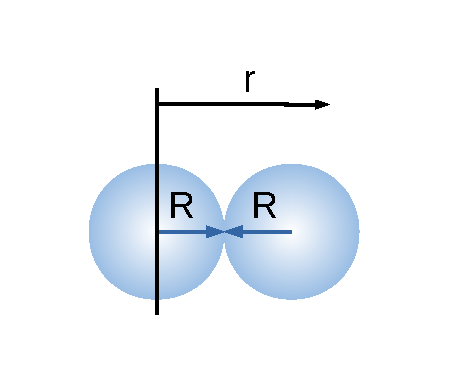
\includegraphics[width=1.1\columnwidth]{figs/TwoSpheresandplot.pdf} 
          \end{figure} 	 
	\end{columns}	
\end{frame}

\subsection*{Freezing}
%\begin{frame}{}
	%\begin{columns}[t]
		%\column{.5\textwidth}
        %\vspace{-2em}
        %\begin{block}{}
            %\begin{itemize}
			    %\item Driven by entropy - maximize the entropy of the universe
				%\item Extract energy to freeze %(add energy to melt)  
			%\end{itemize}   
	    %\end{block}
        %\begin{figure}
            %\centering
            %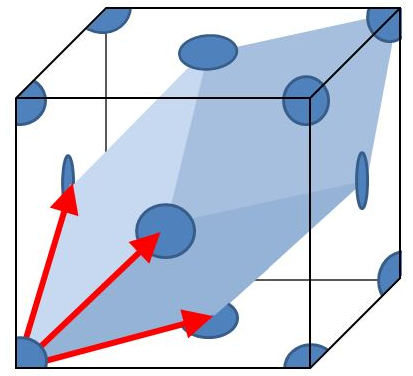
\includegraphics[width=0.4\columnwidth]{PrimitiveCellLightBlue.png}
            %%\caption{Primitive Cell (in blue)}
          %\end{figure}
          %$~~~~~~~$Primitive cell (in blue)
        %\column{.5\textwidth}
	    %\vspace{-1em}
		%\begin{block}{Crystalline Structure}
			%\begin{itemize}
			    %\item Structure depends on V(r)
				%\item Face-Center-Cubic cells 
				%\item Filling a box with marbles
				%\item Parallelpiped primitive cell - 
				%smallest unit that reproduces lattice
				%\item One atom per primitive cell, 4 atoms in FCC cell
			%\end{itemize}
		%\end{block}
	%\end{columns}	
%\end{frame}

%\begin{frame}{Freezing of a WCA Fluid}
	%\begin{columns}[t]
		%\column{.5\textwidth}
	    %%\vspace{-3em}
		%\begin{block}{Freezing...}
		     %\begin{itemize}
				%\item Driven by entropy?				
				%\item Abrupt change in density
				%\item Liquid and solid coexist
			%\end{itemize}		
		%\end{block}
	    %\column{.5\textwidth}
		%\begin{block}{At Freezing ...}
		     %\begin{itemize}
				%\item Thermal equilibrium 
				
				%($\text{T}_{Liquid}$ = $\text{T}_{Solid}$)
			    %\item Mechanical equilibrium 
			    
			    %($\text{P}_{Liquid}$ = $\text{P}_{Solid}$)
				%\item Diffusive equilibrium 
				
				%($\mu_{Liquid}$ = $\mu_{Solid}$)
			%\end{itemize}		
		%\end{block}		
	%\end{columns}	
%\end{frame}

%\subsection*{Phase Diagrams}
\begin{frame}{Freezing of a WCA Fluid}
	\begin{columns}[t]
		\column{.5\textwidth}
	    \vspace{-1em}
		\begin{block}{Phase Transitions}
		     \begin{itemize}
				%\item Driven by entropy - maximize the entropy of the universe				
				\item Abrupt change in density
				
				across coexistence region
			 \end{itemize}		
		\end{block} 
		\begin{block}{WCA Phase Diagram}
		     \begin{itemize}
				\item No attraction	- so no
				
				liquid/gas boundary
				\item Fluid is homogeneous (has
				
				uniform average n spatially) 
				\item "Solid" is a strongly 
				
				inhomogeneous fluid 
				
				with long-range order		
			  \end{itemize}				 
		\end{block}			       
		\column{.5\textwidth}
	    \vspace{-2em}
		 \begin{figure}
            \centering
            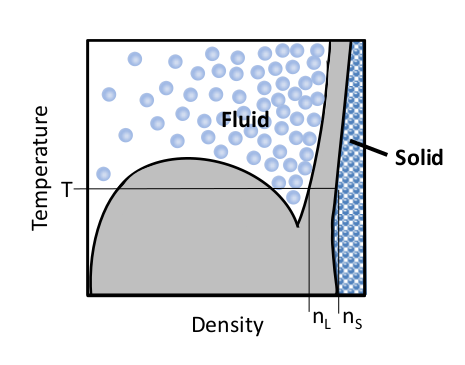
\includegraphics[width=1.1\columnwidth]{figs/T-n_Diagram.pdf}
            %\caption{}
          \end{figure}
          \vspace{-1em}
         $~~~~~~~~~~$ T-n Phase Diagram  
       
	\end{columns}
    \vspace{+1em}
\end{frame}

\begin{frame}{Freezing of a WCA Fluid}
	\begin{columns}[t]
		\column{.5\textwidth}
	    \vspace{-0.5em}
         \begin{block}{At Phase Transition}
		     \begin{itemize}
				\item Thermal equilibrium 
				
				($\text{T}_{Liquid}$ = $\text{T}_{Solid}$)
			    \item Mechanical equilibrium 
			    
			    ($\text{P}_{Liquid}$ = $\text{P}_{Solid}$)
				\item Diffusive equilibrium 
				
				($\mu_{Liquid}$ = $\mu_{Solid}$)
			\end{itemize}		
		\end{block}	
		\begin{block}{WCA Phase Diagram}
		     \begin{itemize}
				\item No liquid/gas boundary				
			  \end{itemize}				 
		\end{block}	
		\column{.5\textwidth}
	    \vspace{-1.5em}
		\begin{figure}
            \centering
            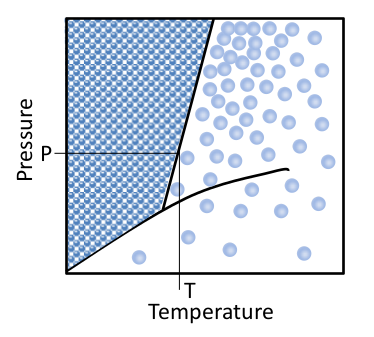
\includegraphics[width=\columnwidth]{figs/P-T_Diagram.pdf}
            %\caption{}
         \end{figure} 
	    \vspace{-1em}                  
         $~~~~~~~~~~$P-T Phase Diagram
	\end{columns}
    \vspace{+1em}	
\end{frame}



%KEEP -------
%\begin{frame}{Freezing of a WCA Fluid}
	%\begin{columns}[t]
		%\column{.5\textwidth}
	    %\vspace{-3em}
		%\begin{block}{}
		     %\begin{itemize}
				%\item Driven by entropy 
				%\item Abrupt change in density
				%\item Liquid and solid coexist
			%\end{itemize}		
		%\end{block}
		%\begin{block}{At Freezing ...}
		     %\begin{itemize}
				%\item Thermal equilibrium 
				
				%($\text{T}_{Liquid}$ = $\text{T}_{Solid}$)
			    %\item Mechanical equilibrium 
			    
			    %($\text{P}_{Liquid}$ = $\text{P}_{Solid}$)
				%\item Diffusive equilibrium 
				
				%($\mu_{Liquid}$ = $\mu_{Solid}$)
			%\end{itemize}		
		%\end{block}		
		%\column{.5\textwidth}
	    %\vspace{-1.5em}
		%\begin{block}{WCA Fluid forms crystals}
			%\begin{itemize}
				%\item Face-Center-Cubic cells 
				%\item Filling a box with marbles
				%\item Parallelpiped primitive cell - 
				%smallest unit that reproduces lattice (shown in blue)
				%\item One atom per primitive cell
			%\end{itemize}
		%\end{block}
        %\begin{figure}
            %\centering
            %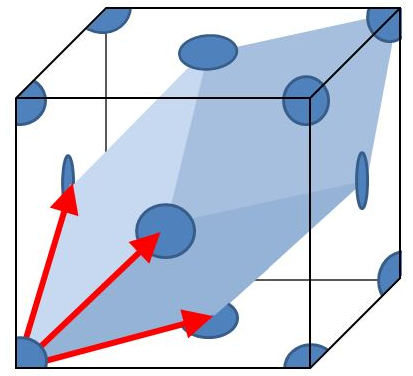
\includegraphics[width=0.4\columnwidth]{PrimitiveCellLightBlue.png}
            %%\caption{Primitive Cell (in blue)}
          %\end{figure}
	%\end{columns}	
%\end{frame}


%\begin{frame}{Conceptual Phase Diagrams}
    %\begin{figure}
        %\centering
        %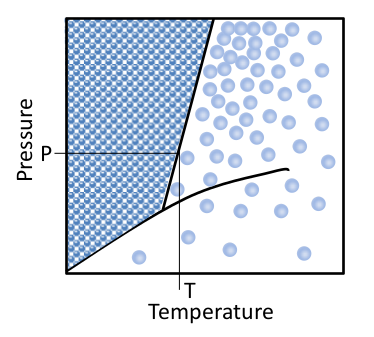
\includegraphics[height=6cm]{figs/P-T_Diagram.pdf}
        %%\caption{Conceptual Pressure-Temperature Phase Diagram}
        %\label{fig:P-T_Diagram}
     %\end{figure}
%\end{frame}

%KEEP------
%\subsection*{Phase Diagrams}
%\begin{frame}{Conceptual Phase Diagrams}
	%\begin{columns}[t]
		%\column{.5\textwidth}
        %\begin{figure}
            %\centering
            %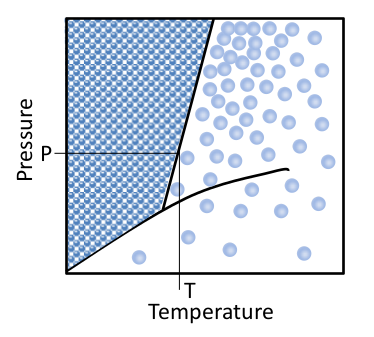
\includegraphics[width=.9\columnwidth]{figs/P-T_Diagram.pdf}
            %%\caption{}
          %\end{figure}
		%\column{.5\textwidth}
		 %\begin{figure}
            %\centering
            %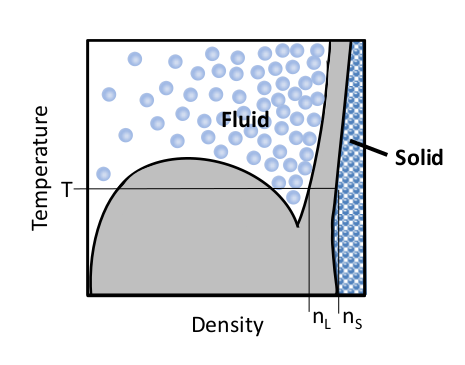
\includegraphics[width=\columnwidth]{figs/T-n_Diagram.pdf}
            %%\caption{}
          %\end{figure}
	%\end{columns}
    %\vspace{+1em}
%Expect WCA phase diagrams to look like these - and not like these.	
%\end{frame}

\subsection*{Finding coexistence}
\begin{frame}{Find Pressure and Number Densities at  Phase Transition}
	\begin{columns}[t]
		\column{.5\textwidth}
		\vspace{-2em}
		\begin{block}{}
			   %\begin{displaymath}{P = -\frac{\partial{f}}{\partial{\frac{1}{n}}}\bigg|_{T,N}}\end{displaymath} 
				%\begin{displaymath} \mu = f + \frac{1}{n}P\end{displaymath}
			\begin{itemize} 
                 \item Phase transition pressure at point where $P_L=P_S$ and $\mu_L=\mu_S$ for a given T							
			     %\item Phase transition liquid and solid number densities found at phase transition pressure
			     %item Find Helmholtz free energy
			     \vspace{+1em}
			     \item Helmholtz free energy per atom, $f=\frac{F}{N}$ at T, n gives

				 %\item %Pressure = -slope								
				 \begin{displaymath}{P = -\frac{\partial{f}}{\partial{\frac{1}{n}}}\bigg|_{T,N}}\end{displaymath} 
				 %\item %$\mu$ = y-intercept
				 \begin{displaymath} \mu = f + \frac{1}{n}P\end{displaymath}		
				 Find pressure at intersection 		
			\end{itemize}
	    \end{block}	    
	    \column{.55\textwidth}
		\vspace{-2em}
            \begin{figure}
                \centering
                %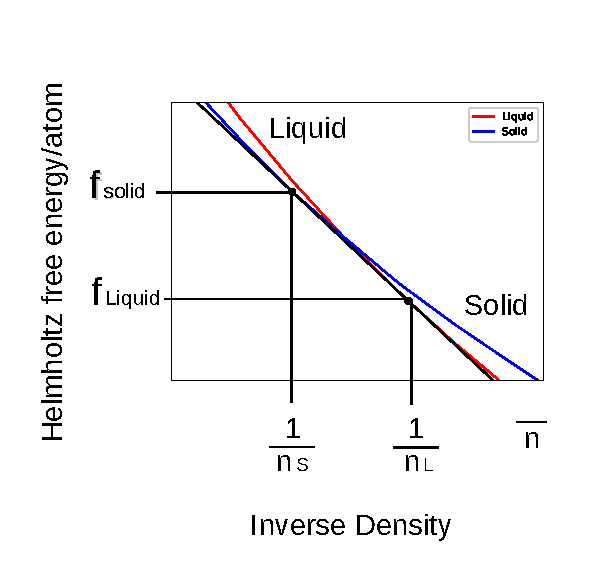
\includegraphics[width=1.2\columnwidth]{figs/MaxwellDTC-Fig1-realplot.pdf}
                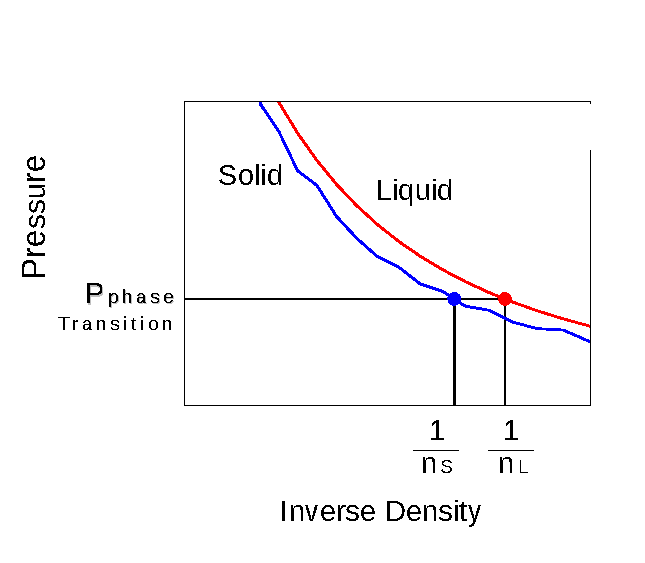
\includegraphics[width=0.9\columnwidth]{figs/MaxwellDTC-Fig3-realplot.pdf}
            \end{figure}
            \vspace{-.5em}
			\begin{itemize} 						
			    \item Phase transition liquid and solid number densities, $\text n_L$ and $\text n_S$ found at $\text P_{phase.transition}$
			\end{itemize}
            
            %\textcolor{blue}{$~~~~~~~~~~~\rightarrow$ Find Helmholtz free energy}
	\end{columns}	
\end{frame}

%\begin{frame}
%\begin{frame}{Maxwell's Double Tangent Construction}
	%\begin{columns}[t]
		%\column{.5\textwidth}
		%\vspace{-0.5em}
		%\begin{block}{$~~~$Find liquid and solid 
		
		%$~~~$number densities 
		
		%$~~~$at the phase transition}
			%\begin{itemize}
				%\item Data from cDFT 
				%\item Temperature fixed
				%\item Pressure = -slope
				%%\item $\mu$ = y-intercept
			%\end{itemize}
	    %\end{block}
	    %\begin{displaymath}{P = -\frac{\partial{f}}{\partial{\frac{1}{n}}}\bigg|_{T,N}}\end{displaymath} 
	    %\column{.65\textwidth}
		%\vspace{-4em}
            %\begin{figure}
                %\centering
                %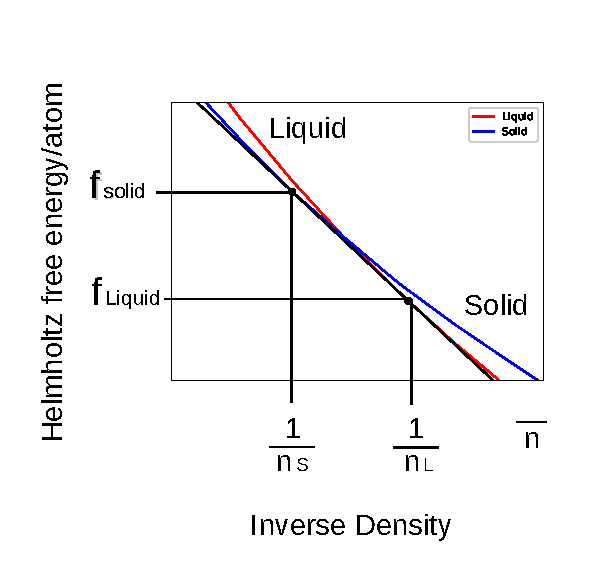
\includegraphics[width=1.2\columnwidth]{figs/MaxwellDTC-Fig1-realplot.pdf}
            %\end{figure}
	%\end{columns}	
%\end{frame}

%\begin{frame}{Maxwell's Double Tangent Construction}
	%\begin{columns}[t]
		%\column{.5\textwidth}
        %\begin{figure}
            %\centering
            %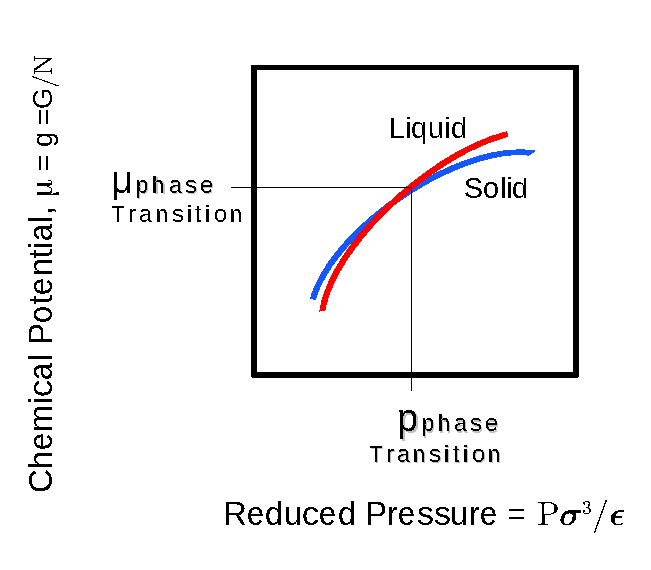
\includegraphics[width=\columnwidth]{figs/MaxwellDTC-Fig2.pdf}
          %\end{figure}
		%\column{.5\textwidth}
		%\begin{block}{At Phase Transition}
			%\begin{itemize}
				%\item $\text{T}_{Liquid}$ = $\text{T}_{Solid}$
			    %\item $\text{P}_{Liquid}$ = $\text{P}_{Solid}$
				%\item $\mu_{Liquid}$ = $\mu_{Solid}$
			%\end{itemize}
	    %\end{block}
	    %\begin{block}{Plot $\mu$ vs P }
			%\begin{itemize}
				%\item Pressure at phase transition found
				%from intersection
			%\end{itemize}
		%\end{block}
	%\end{columns}	
%\end{frame}

%\begin{frame}{Maxwell's Double Tangent Construction}
	%\begin{columns}[t]
		%\column{.5\textwidth}
        %\begin{figure}
            %\centering
            %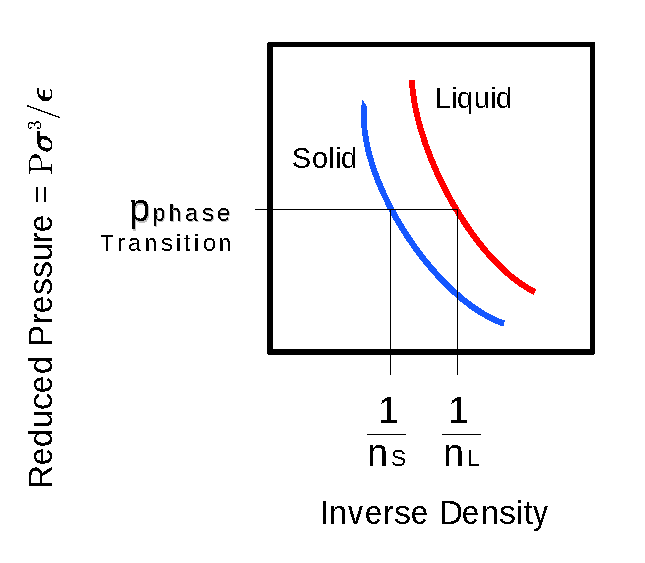
\includegraphics[width=\columnwidth]{figs/MaxwellDTC-Fig3.pdf}
          %\end{figure}
		%\column{.5\textwidth}
		%\begin{block}{Identify phase transition...}
			%\begin{itemize}
				%\item Liquid number density
				%\item Solid number density
			%\end{itemize}
		%\end{block}
		%\begin{block}{Construct phase diagrams}
	    %\end{block}
	%\end{columns}	
%\end{frame}

\begin{frame}{Helmholtz Free Energy Breaks into Two Parts}
    \begin{block}{}
        \vspace{-2em}
        \begin{displaymath}F=F_{ideal} + F_{excess}\end{displaymath}
        \vspace{-.7em}        
        \begin{itemize}            
           \item Ideal - \textcolor{blue}{EASY} to find - does not depend on V(r) 
           \begin{displaymath}F_{ideal}[n(\vec{r})]= k_BT\int_{Vol}[n(\vec{r})\ln(n(\vec{r})/\text{n}_\text{Q})-n(\vec{r})]d\vec{r}\end{displaymath}
           \vspace{+0.01em} 
           \item Excess - \textcolor{red}{HARD} to find - depends on V(r) 
           
        \vspace{+1.5em} 
            $~~~~~~~$Classical Density Functional Theory (cDFT) is 
            
            $~~~~~~~$our way out of this problem!
            %\small Simplified expression in terms of Mayer function, 
            %\footnotesize $f(r)=e^{-\frac{V(r)}{k_{B}T}}-1$ for pairs of atoms is:
        \end{itemize}
        %%\vspace{+0.02em} 
        %\footnotesize
        %%
        %\begin{displaymath} 
             %F_{excess}=-k_BT\ln{\left(\frac{1}{V^N}\int{...}\int d\vec r^1{...}d\vec r^N \left[1 + \sum{f_{ij}} + \sum{f_{ij}f_{kl}}                        
             %+\sum{f_{ij}f_{kl}f_{mn}} +... \right]\right)}
        %\end{displaymath}
        %\normalsize
     \end{block}
\end{frame}


\section*{Classical density functional theory}
\subsection*{cDFT}
\begin{frame}{First Key Idea in Classical Density Functional Theory}
    %\vspace{+1em} 
    \begin{block}{1) Free energy can be written as functional $\text f[\text{n}(\vec r)]$}  
       \begin{itemize}
          \item A functional is a function of a function (ie. integral)
          \item Number density profile, $\text n(\vec{r})$ is an ensemble average
          %\item Number density, n is number of atoms per volume $\text n=\frac{\text N}{\text V}$
          
           that describes how number density varies spatially on average. 
          \begin{displaymath}\text n(\vec r)=~\left<\sum_{i=1}^{\text N}\delta(\vec r - \vec r_i)\right>~\end{displaymath} 
          \begin{displaymath} \text n=\frac{1}{\text V}\int_{vol}{\text n(\vec{r})}{d\vec{r}}=\frac{\text N}{\text V}\end{displaymath}
        \end{itemize}
    \end{block}
\end{frame}  
  
\begin{frame}{Second Key Idea Classical Density Functional Theory}
    %\vspace{+1em}    
    \begin{block}{2) Free energy tends toward a minimum at equilibrium }
    \begin{itemize}
       %\item Minimize the Helmholtz free energy
       %\item Form Functional using SFMT
	   %\item Free energy written as a functional of a number density profile $\text f[\text{n}(\vec r)]$       
       %\item Free energy tends toward a minimum at equilibrium 
       %\item Vary $\text n(\vec{r})$ until the free energy is minimized 
       %\item Equilibrium Free Energy found!
       \item For a closed system (energy conserved)
       \item As the entropy of the universe is maximized
       \item While holding natural variables FIXED
    \end{itemize}
    
       %Natural variables for Helmholtz free energy F(T,V,N) are Temperature, Volume, and Number of particles
       Natural variables for Helmholtz free energy per atom,          %good-keep 
       f(T,$\frac{V}{N}$) are temperature and specific volume (or inverse number density). 
       %f(T,$\frac{1}{n}$) are temperature and inverse number density. %good-keep 
       %\begin{displaymath}df=\frac{\partial f}{\partial T}dT + \frac{\partial f}{\partial \frac{1}{n}}d\left(\frac{1}{n}\right)\end{displaymath}    %good-keep 
       %\begin{displaymath} \text{df}_{\text{System}}=-\left(\frac{\text T}{\text N}\right)\text{dS}_{\text{System+Surroundings}} \end{displaymath}  %good-keep
     \end{block}     
\end{frame}

\begin{frame}{Classical Density Functional Theory (cDFT)}
    \begin{block}{Implementing cDFT}
    \begin{itemize}
       %\item Minimize the Helmholtz free energy
       %\item Form Functional using SFMT
	   %\item Free energy written as a functional of a number density profile $\text f[\text{n}(\vec r)]$       
       %\item Free energy tends toward a minimum at equilibrium 
       \item Form a functional $\text f[\text n(\vec r)]$
       \item n is fixed, $\text n(\vec{r})$ is set free
       \item Vary $\text n(\vec{r})$ until the free energy is minimized 
       
       Free Energy goes to its equilibrium value when minimized      
       \begin{displaymath}\text f[\text n(\vec r)]\rightarrow \text f_{\text{eq}}[\text n_{\text{eq}}(\vec r)]  \mbox{ as f is minimized} \end{displaymath}
       %and $\text n(\vec{r})$ goes to its equilibrium value as well!
       \begin{displaymath}{\mbox{where }  \text n(\vec{r}) = \text n_{\text{eq}}(\vec r)  \mbox{ at equilibrium}}\end{displaymath}              
       
       %\item Equilibrium Free Energy and number density profile found!
       %\item equilibrium free energy and equilibrium number density profile
     \end{itemize} 
     \end{block}
The reason this works is because cDFT satisfies the conditions 
of the variational principle which requires that  $\text f[\text n(\vec r)]$ 
be a unique functional of  $\text n_{\text{eq}}(\vec{r})$, and that it has 
minimum extremum at $\text n_{\text{eq}}(\vec{r})$.
\end{frame}


%%\subsection*{SPT}
%\begin{frame}{Scaled Particle Theory}
  %SPT
%\end{frame}

%%\subsection*{FMT}
%\begin{frame}{Fundamental Measure Theory}
  %SPT
%\end{frame}

\subsection*{SFMT}
\begin{frame}{Soft Fundamental Measure Theory}
%   \begin{block}{Scaled Particle Theory (SPT)}
%        \begin{itemize}
%            \item Finds $F_{excess}$ for a homogeneous (uniform number density)
%            hard-sphere fluid
%        \end{itemize}
%   \end{block}
  \begin{block}{Fundamental Measure Theory (FMT)} 
       \begin{itemize}
           \item cDFT for hard spheres developed by Rosenfeld
           \item Based on \structure{weighted densities}, involving
                 ``fundamental measures'' like the surface area
           \item Weighting functions such as Dirac $\delta$-function shells
       \end{itemize}
  \end{block} 
  \begin{block}{SFMT}
     \begin{itemize}            
           \item Developed by Schmidt, extension of FMT 
           \item Finds $F_{excess}$ for an inhomogeneous soft-sphere fluid
           \item Smooth weighting functions for
                continuous ``soft'' potentials
     \end{itemize}
  \end{block}  
    %More coming soon .... Schmidt's and Rosenfeld's secret sauce
\end{frame}

\subsection*{Our WCA Functional}
%\begin{frame}
%\begin{frame}{Our WCA Functional}
    %%\small
    %\begin{align}\label{eq:Fexfunctional}
        %F_{excess}[\textcolor{blue}{\text{n}(\vec{r})}]=k_BT\int(\Phi_1(\vec{r})+\Phi_2(\vec{r})+\Phi_3(\vec{r}{)) d}\vec{r}
     %\end{align}
     %%where 
     %\begin{align}
         %\Phi_1 &= -n_{0}\ln(1-n_{3}) \\
         %\Phi_2 &= \frac{n_{1}n_{2}-\vec{n_{1}}\cdot\vec{n_{2}}}{1-n_{3}} \\
         %\Phi_3 &= \frac{{n_2}^3-3n_2\vec{n}_{v2}\cdot\vec{n}_{v2}+\frac{9}{2}[\vec{n}_{v2}\cdot{\overleftrightarrow{n}_{m2}}\cdot{\vec{n}_{v2}}-\operatorname{Tr}({\overleftrightarrow{n}^3_{m2}})]}{24\pi(1-n_3)^2}  
      %\end{align} 
      %\begin{align}\label{eq:numdenprofile}
	      %n_i(\vec{r})=\int_{Volume}{\textcolor{blue}{\text n(\vec{r'})}w_i(|\vec{r}-\vec{r'}|)d{\vec{r'}}}
      %\end{align}
      %%\begin{align}\label{eq:weights}
  %%w_{0}(r) &=\frac{w_{2}}{4\pi{r}^2} \\
  %%w_{1}(r) &=\frac{w_{2}}{4\pi{r}} \\
  %%w_2(r) &=-\frac{\partial{w_3(r)}}{\partial{r}} \\
  %%&= \frac{\sqrt{2}}{\Xi\sqrt\pi}\exp^{-\left(\frac{r-\frac{\alpha}{2}}{\Xi/\sqrt{2}}\right)^2}  \\
  %%w_3(r) &=\frac{1}{2}\left[1-\operatorname{erf}\left(\frac{r-\frac{\alpha}{2}}{\frac{\Xi}{\sqrt{2}}}\right)\right]  
%%\end{align}
%%\begin{equation}\label{eq:w_v2}{  \vec{w_{2}}=w_{2}\frac{\vec{r}}{r}  }\end{equation}
%%\begin{equation}\label{eq:w_v1}{  \vec{w_{1}}=w_{1}\frac{\vec{r}}{r}  }\end{equation} 
%%\begin{equation}\label{eq:tensorweight-methods}\overleftrightarrow{w}_{m2}(\vec{r}) = w_2(r)\left(\frac{\vec{r}\vec{r}}{r^2}-\frac{I}{3}\right)\end{equation}
%\normalsize
%\end{frame}

\begin{frame}{Our weighting function}
    \begin{itemize}
        \item All the weighting functions can be derived from $w_2(r)$
        \item $w_2$ is related to $V(r)$ by
        \begin{align}
          %\frac{df}{dr} &= 
          -\beta \frac{dV}{dr}e^{-\beta V(r)}
             = \int_{-\infty}^{\infty}w_2(r')w_2(r-r')dr'
      \end{align}
      but this equation is hard to solve
      \item Following Schmidt, we approximate $w_2$ by as a gaussian
      %\begin{displaymath}w_2(r)=\frac{\sqrt{2}}{\Xi\sqrt\pi}\exp^{-\left(\frac{r-\frac{\alpha}{2}}{\Xi/\sqrt{2}}\right)^2}\end{displaymath}
    %   \begin{align}\label{eq:weights}
    %       w_2(r) % &=-\frac{\partial{w_3(r)}}{\partial{r}}
    %        = \frac{\sqrt{2}}{\textcolor{red}{\Xi}\sqrt\pi}\exp^{-\left(\frac{r-\frac{\textcolor{red}{\alpha}}{2}}{\textcolor{red}{\Xi}/\sqrt{2}}\right)^2}
    %   \end{align}
      \item Adjust parameters $\alpha$ and $\Xi$ to approximate the above relation with a resluting $V(r)$
that gives the correct second virial coefficient of a WCA fluid at each temperature
      %\begin{displaymath}w_2(r)=\frac{\sqrt{2}}{\Xi\sqrt\pi}\exp^{-\left(\frac{r-\frac{\alpha}{2}}{\Xi/\sqrt{2}}\right)^2}\end{displaymath}
    \end{itemize}
    %\small
    %\begin{align}\label{eq:Fexfunctional}
        %F_{excess}[\text{n}(\vec{r})]=k_BT\int(\Phi_1(\vec{r})+\Phi_2(\vec{r})+\Phi_3(\vec{r}{)) d}\vec{r}
     %\end{align}
     %%where 
     %\begin{align}
         %\Phi_1 &= -n_{0}\ln(1-n_{3}) \\
         %\Phi_2 &= \frac{n_{1}n_{2}-\vec{n_{1}}\cdot\vec{n_{2}}}{1-n_{3}} \\
         %\Phi_3 &= \frac{{n_2}^3-3n_2\vec{n}_{v2}\cdot\vec{n}_{v2}+\frac{9}{2}[\vec{n}_{v2}\cdot{\overleftrightarrow{n}_{m2}}\cdot{\vec{n}_{v2}}-\operatorname{Tr}({\overleftrightarrow{n}^3_{m2}})]}{24\pi(1-n_3)^2}  
      %\end{align} 
    %   \begin{align}\label{eq:weights}
        %   w_{0}(r) &=\frac{w_{2}}{4\pi{r}^2} \\
        %   w_{1}(r) &=\frac{w_{2}}{4\pi{r}} \\
        %   w_2(r) % &=-\frac{\partial{w_3(r)}}{\partial{r}}
        %    = \frac{\sqrt{2}}{\textcolor{red}{\Xi}\sqrt\pi}\exp^{-\left(\frac{r-\frac{\textcolor{red}{\alpha}}{2}}{\textcolor{red}{\Xi}/\sqrt{2}}\right)^2}  \\
        %   w_3(r) &= \frac{1}{2}\left[1-\operatorname{erf}\left(\frac{r-\frac{\textcolor{red}{\alpha}}{2}}{\frac{\textcolor{red}{\Xi}}{\sqrt{2}}}\right)\right]  
    %   \end{align}
% \begin{equation}\label{eq:w_v2}  \vec{w_{2}}=w_{2}\frac{\vec{r}}{r}  {~~~~~~~~~~}\vec{w_{1}}=w_{1}\frac{\vec{r}}{r} \end{equation}
% %\begin{equation}\label{eq:w_v2}  \vec{w_{2}}=w_{2}\frac{\vec{r}}{r}  \end{equation}
% %\begin{equation}\label{eq:w_v1}  \vec{w_{1}}=w_{1}\frac{\vec{r}}{r}  \end{equation} 
% \begin{equation}\label{eq:tensorweight-methods}\overleftrightarrow{w}_{m2}(\vec{r}) = w_2(r)\left(\frac{\vec{r}\vec{r}}{r^2}-\frac{\text I}{3}\right)\end{equation}
% \normalsize
\end{frame}

%\begin{frame}
%\begin{frame}{Our WCA Functional}
    %\small
     %Evaluate:
    %\begin{equation} \frac{df(r)}{dr}=\int_{-\infty}^{\infty}{w_2(r')w_2(r-r')dr'}\end{equation}
    %%\begin{displaymath}{\frac{df(r)}{dr}=\frac{1}{\Xi\sqrt{\pi}}e^{-\left(\frac{r-\alpha}{\Xi}\right)^2}}\end{displaymath} 
    %% integrate
    %\begin{displaymath}{f(r)=\int_{\infty}^r{ \frac{1}{\textcolor{red}{\Xi}\sqrt{\pi}}e^{-\left(\frac{r'-\textcolor{red}{\alpha}}{\textcolor{red}{\Xi}}\right)^2}{dr'}}}\end{displaymath} 
    %$V_{erf}(r)$  Mayer function:
    %\begin{equation} f(r)=-\frac{1}{2}\left[1-\operatorname{erf}\left(\frac{r-\textcolor{red}{\alpha}}{\textcolor{red}{\Xi}}\right)\right]\end{equation} 
    %%the Mayer function is
    %\begin{displaymath}f(r)=e^{-\frac{V(r)}{K_BT}}-1\end{displaymath} 
    %\begin{equation} 
        %V_{erf}(r)=-k_BT\ln\left[\frac{1}{2}\left(\operatorname{erf}\left(\frac{r-\textcolor{red}{\alpha}}{\textcolor{red}{\Xi}}\right)+1\right)\right]
    %\end{equation} 
        %\normalsize      
%\end{frame}

\begin{frame}{Determine alpha, $\alpha{(}T)$}
	\begin{columns}[t]
		\column{.5\textwidth}
	    \vspace{-01em}
		\begin{block}{}
			\begin{itemize}
			    %\item $V_{erf}$ is temperature dependent, $V_{WCA}$ is not
			    \item Make $V(r)=V_{WCA}(r)$ at $r=\alpha$ where 
			    the convolution of w2 with itself is greatest
			    \item Ideally, curves would match
			    %\item $\alpha$ decreases with temperature 
			    %\item radius of weight functions equal to $\alpha/2$
			\end{itemize}
				\vspace{-0.5em}
			   \begin{figure}
                   \centering
                   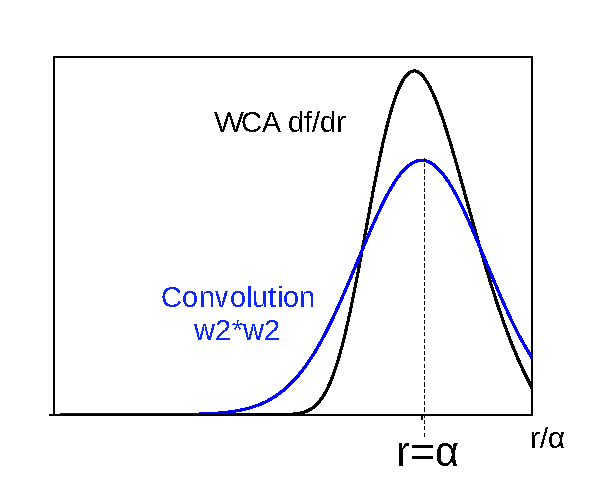
\includegraphics[width=.9\columnwidth]{figs/df_dr_with_xi_fromB2_pic.pdf}
                   %\includegraphics[width=.7\columnwidth]{plot_alpha.pdf}
                   %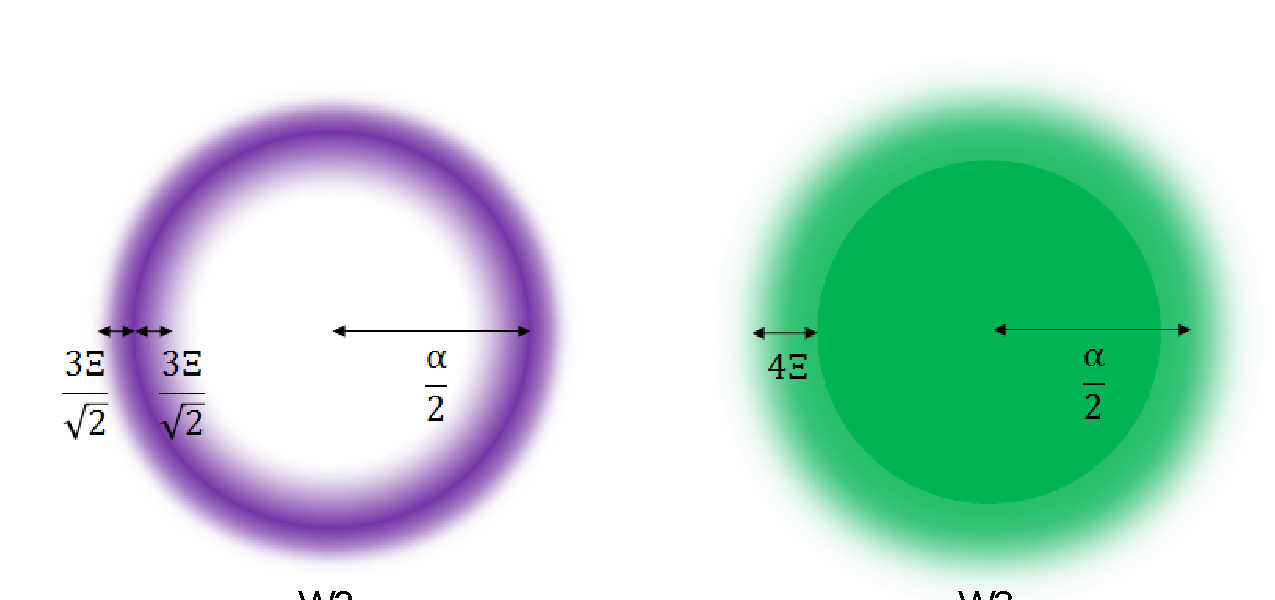
\includegraphics[width=.7\columnwidth]{figs/w2-w3.pdf}
                \end{figure}
		\end{block}	  
		\column{.55\textwidth}
        \vspace{-0.5em}
        \begin{block}{}
        %\vspace{-1em}	
        \begin{itemize}
			    %\item $V_{erf}$ is temperature dependent, $V_{WCA}$ is not
			    %\item Make $V(r)=V_{WCA}(r)$ at $r=\alpha$ where 
			    %the convolution of w2 with itself is greatest
			    %\item Ideally, would like these curves to match
			    \item $\alpha$ decreases with temperature 
			    \item $\alpha$ is related to the radius of weight functions
			\end{itemize}
        \begin{figure}
            \centering
            %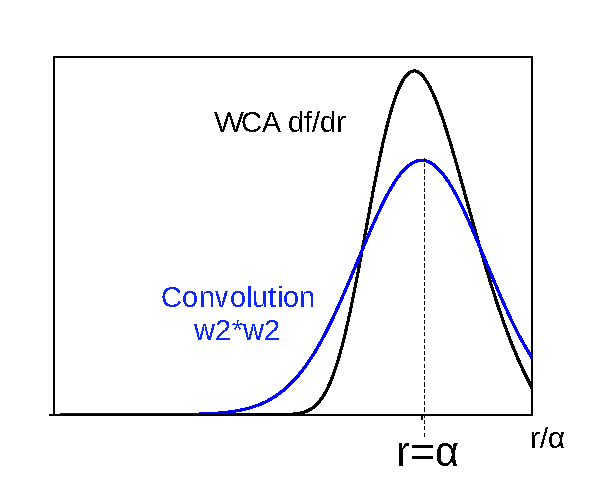
\includegraphics[width=\columnwidth]{figs/df_dr_with_xi_fromB2_pic.pdf}
            %\includegraphics[width=.7\columnwidth]{plot_alpha.pdf}
            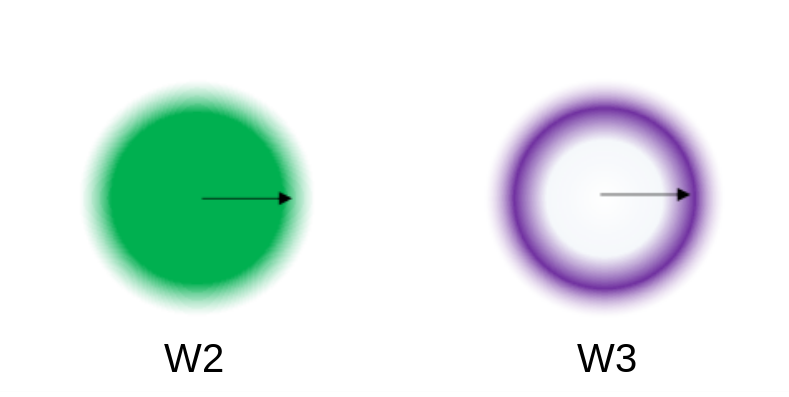
\includegraphics[width=\columnwidth]{figs/w2-w3-radius.png}
          \end{figure}
	    \end{block}          
	\end{columns}	
\end{frame}


\begin{frame}{Determine Xi, $\Xi{(}T)$}
	\begin{columns}[t]
		\column{.5\textwidth}
	    \vspace{-0.5em}
		\begin{block}{}
            \begin{itemize}
			    \item Match 2nd Virial Coefficients
			\end{itemize}
		    %\vspace{+0.5em}
		    
		    \begin{displaymath}B_2=-\frac{1}{2}\int_{Volume} e^{-\frac{V(r)}{k_{B}T}}-1~d\vec r\end{displaymath} 					    
		     %\vspace{+0.5em}
		     
			\begin{displaymath}B_{2\operatorname{V(r)}}(T) =B_{2WCA}(T)\end{displaymath}         
	        %\item $\Xi$ increases with temperature 
			%\item $\Xi$ is related to the thickness of weight functions	    
	    \end{block}
		%\vspace{-1em}
		\column{.5\textwidth}
        \vspace{-0.5em}       
        %\begin{figure}
            %\centering
            %\includegraphics[width=.7\columnwidth]{xi_fromB2.pdf}
          %\end{figure}            
        \vspace{-0.5em}
        \begin{block}{}
        %\vspace{-1em}	
        \begin{itemize}
			    %\item $V_{erf}$ is temperature dependent, $V_{WCA}$ is not
			    %\item Make $V(r)=V_{WCA}(r)$ at $r=\alpha$ where 
			    %the convolution of w2 with itself is greatest
			    %\item Ideally, would like these curves to match
			    \item $\Xi$ increases with temperature 
			    \item $\Xi$ is related to the thickness of weight functions
			\end{itemize}
	    \vspace{-2em} 
        \begin{figure}
            \centering
            %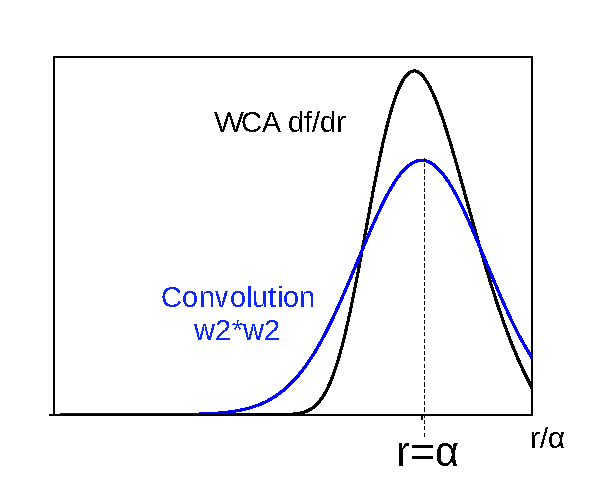
\includegraphics[width=\columnwidth]{figs/df_dr_with_xi_fromB2_pic.pdf}
            %\includegraphics[width=.7\columnwidth]{plot_alpha.pdf}
            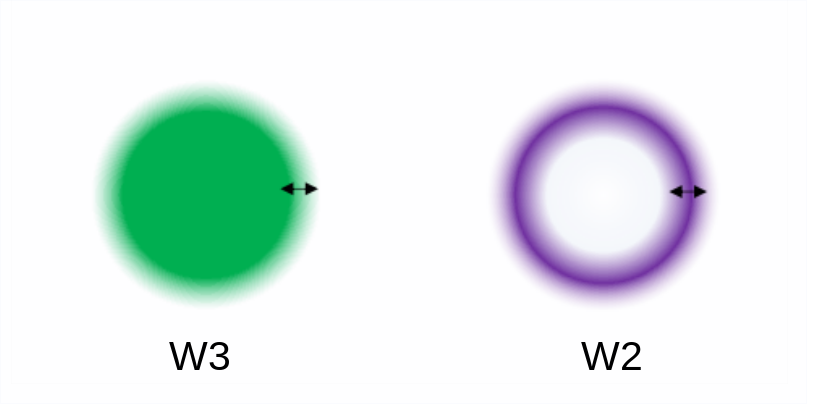
\includegraphics[width=1.1\columnwidth]{figs/w2-w3-thickness.png}
          \end{figure}
	    \end{block}              
	\end{columns}	
\end{frame}



\section*{Identifying freezing}
\subsection*{Density of a crystal}

\begin{frame}{Classical Density Functional Theory (cDFT)}
    \begin{block}{Implementing cDFT}
    \begin{itemize}
       %\item Minimize the Helmholtz free energy
       %\item Form Functional using SFMT
	   %\item Free energy written as a functional of a number density profile $\text f[\text{n}(\vec r)]$       
       %\item Free energy tends toward a minimum at equilibrium 
       \item Form a functional $\text f[\text n(\vec r)]$  \checkmark
       \item n is fixed, $\text n(\vec{r})$ is set free \textcolor{red}{$\rightarrow$ need to create many $\text n(\vec{r})$}
       \item Vary $\text n(\vec{r})$ until the free energy is minimized 
       
       Free Energy goes to its equilibrium value when minimized      
       \begin{displaymath}\text f[\text n(\vec r)]\rightarrow \text f_{\text{eq}}[\text n_{\text{eq}}(\vec r)]  \mbox{ as f is minimized} \end{displaymath}
       %and $\text n(\vec{r})$ goes to its equilibrium value as well!
       \begin{displaymath}{\mbox{where }  \text n(\vec{r}) = \text n_{\text{eq}}(\vec r)  \mbox{ at equilibrium}}\end{displaymath}              
       
       %\item Equilibrium Free Energy and number density profile found!
       %\item equilibrium free energy and equilibrium number density profile
     \end{itemize} 
     \end{block}
\end{frame}

%\begin{frame}{}
%\begin{figure}
       %\centering
       %\includegraphics[height=4cm]{Simple_cell.png}
       %A simplified cell
 %\end{figure} 
%\end{frame}

%\begin{frame}{}
    %\begin{itemize}
	    %\item Atoms not exactly on lattice sites
		%\item Gaussian distribution results
		%\item Number density = 1 atom per bold-box volume
	%\end{itemize}	
	
    %\begin{figure}
       %\centering
       %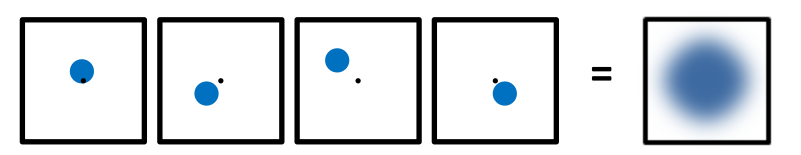
\includegraphics[height=2cm]{Ensemble_Gaussian.png}
       %%\caption{On the left are shown four examples of possible positions 
       %%that an atom (blue sphere) might have within a cell that has one 
       %%lattice site (black dot) at the center. A large number of such 
       %%possibilities would give rise to a Gaussian distribution, 
       %%as shown on the right.}
       %\label{fig:Ensemble_Gaus}
        %Front view of an atom in a simplified cell
     %\end{figure}     
%\end{frame}	

%\begin{frame}{A Gaussian Distribution}
    %\begin{figure}
       %\centering
       %\includegraphics[height=5cm]{Gaussian}
       %%\caption{A 2D Gaussian Distribution of width 2$\sigma$}
       %\label{fig:Gaus_plot}
       
       %A 2D Gaussian Distribution of width 2$\sigma$
    %\end{figure}  
    
%\end{frame}

%\begin{frame}{}
    %\begin{itemize}
	    %\item Not all lattice sites are occupied
		%\item More Gaussian Distributions, but shorter
		%\item Number density = 1 atom per bold-box volume
	%\end{itemize}	

    %\begin{figure}
       %\centering
       %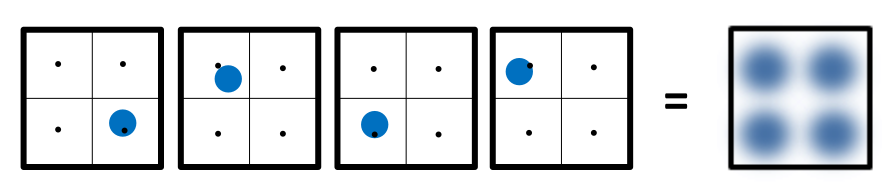
\includegraphics[height=2cm]{Ensemble_Smallcells.png}
       %%\caption{On the left are shown four examples of possible positions 
       %%that an atom (blue sphere) might have within a fixed volume 
       %%containing eight cells. Each cell has one lattice site at the center 
       %%represented by a black dot. A large number of such possibilities 
       %%would give rise to the Gaussian distributions shown on the right.}
       %\label{fig:Ensemble_Smallcells}
       
       %An atom in a cube consisting of 8 smaller simplified cells
    %\end{figure}     
%\end{frame}

%\begin{figure}
   %\centering
   %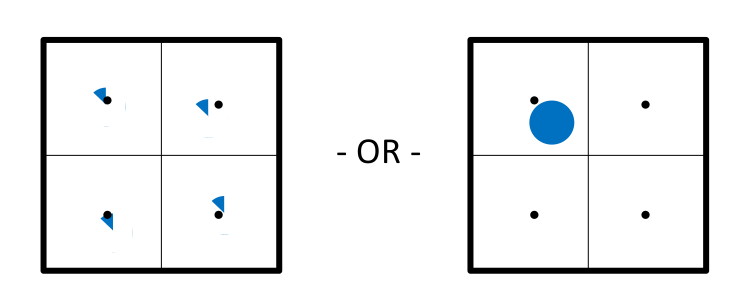
\includegraphics[height=2cm]{SameStatPic.png}
   %%\caption{Front views of a cube with eight smaller cells. The two views 
   %%show two ways of picturing a fraction of vacancies, $f_v$ of 7/8 which 
   %%give rise to the same Gaussian distribution statistically, 
   %%and the same number density.}
   %fraction
   %\label{fig:SameStatPic}
%\end{figure} 


\begin{frame}{Number Density Profiles}
	\begin{columns}[t]
		\column{.5\textwidth}
	    \vspace{-2em}
        \begin{block}{}
            \begin{itemize}
            %\item Gaussian distribution at each lattice site
            \item $\text n(\vec{r})$ is sum of Gaussian 
            
            distributions, each  
            
            centered at a lattice site
            \item Atoms not exactly on lattice
            
            sites, width of 
            Gaussians vary
            \item Not all lattice sites occupied,
            shrink cells as fraction of 
            
            vacancies increase to keep 
            
            number density same
            \item Each $n(\vec r)$ is the equilibrium profile
            valid for some fixed external potential. 
            
            \end{itemize}
        \end{block}
		\column{.65\textwidth}
		\vspace{-2.5em}
		%%\small{$~~~~~~~$Simplified cell}
		    \begin{figure}
               %%\centering
               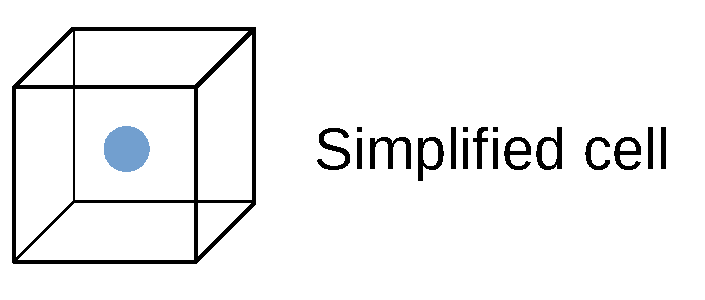
\includegraphics[height=1.5cm]{figs/Simplified_cell.pdf}
            \end{figure}
    \normalsize
             \vspace{-2em} 
    	    \begin{figure}
               \centering
               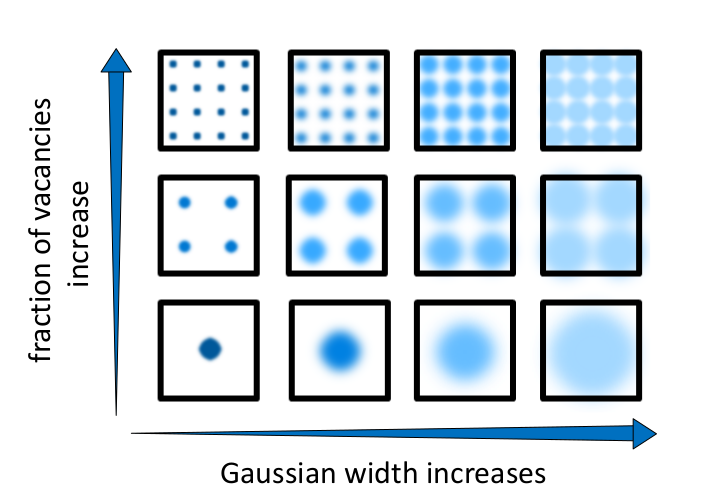
\includegraphics[height=4.5cm]{VaryWidthandVacancies.png}
               %\caption{Number density profiles $n(\vec r)$, all with 
               %the same number density, n.}
            \end{figure} 
             \vspace{-0.5em} 
                \footnotesize
    $~~~~~~~~~~$Many number density profiles $n(\vec r)$, 
    
    $~~~~~~~~~~$all with the same number density, n.
	\end{columns}
\end{frame}

%\begin{frame}{Monte-Carlo Integration}
   %\begin{columns}
		%\column{.5\textwidth}
		%\begin{block}{}
		  %\begin{itemize}
		  %\item 
		  %\item
		  %\end{itemize}
		%\end{block}
	    %\column{.65\textwidth}
	    %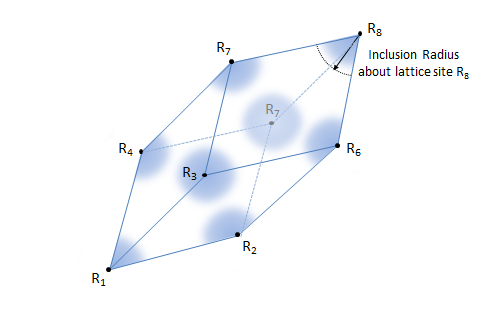
\includegraphics[height=4cm]{InclusionRadius.png}
   %\end{columns}
%\end{frame}

\begin{frame}{Classical Density Functional Theory (cDFT)}
    \begin{block}{Implementing cDFT}
    \begin{itemize}
       %\item Minimize the Helmholtz free energy
       %\item Form Functional using SFMT
	   %\item Free energy written as a functional of a number density profile $\text f[\text{n}(\vec r)]$       
       %\item Free energy tends toward a minimum at equilibrium 
       \item Form a functional $\text f[\text n(\vec r)]$  \checkmark
       \item n is fixed, $\text n(\vec{r})$ is set free $\rightarrow$ create many $\text n(\vec{r})$ \checkmark
       \item \textcolor{red}{Vary $\text n(\vec{r})$ at fixed T until the free energy is minimized} 
       
       Free Energy goes to its equilibrium value when minimized      
       \begin{displaymath}\text f[\text n(\vec r)]\rightarrow \text f_{\text{eq}}[\text n_{\text{eq}}(\vec r)]  \mbox{ as f is minimized} \end{displaymath}
       %and $\text n(\vec{r})$ goes to its equilibrium value as well!
       \begin{displaymath}{\mbox{where }  \text n(\vec{r}) = \text n_{\text{eq}}(\vec r)  \mbox{ at equilibrium}}\end{displaymath}              
    \end{itemize}   
    
       Construct phase diagrams using (f,$\frac{1}{n}$) data for each temperature to find P, $\text n_L, \text n_S$  at phase transitions.
       %Collect (f,$\frac{1}{n}$) data for each temperature T
       %to use in Maxwell's Double Tanget Construction 
       %to get the pressure P,
       %and the liquid and solid number densities $\text n_L, \text n_S$ at the phase transition for each T
       %\item Equilibrium Free Energy and number density profile found!
       %\item equilibrium free energy and equilibrium number density profile
 
     \end{block}
\end{frame}

%Monte-Carlo Integration
%\begin{frame}{Monte-Carlo Integration}
	%\begin{columns}[t]
		%%\column{.5\textwidth}
        %%\begin{figure}
            %%\centering
            %%\includegraphics[width=\columnwidth]{Gaussian}
            %%A 2D Gaussian Distribution of width 2$\sigma$
          %%\end{figure}
		%\column{.5\textwidth}
		 %\begin{figure}
            %\centering
            %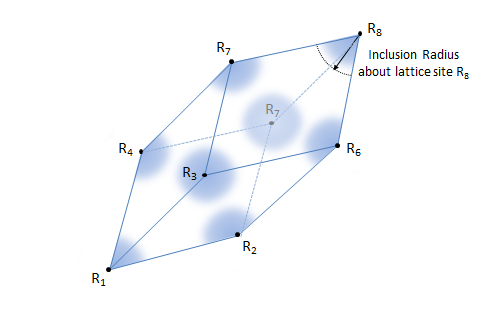
\includegraphics[width=1.02\columnwidth]{InclusionRadius.png}
            %A primitive cell with Gaussians at lattice sites
          %\end{figure}
	%\end{columns}		
%\end{frame}


%\begin{figure}
   %\centering
   %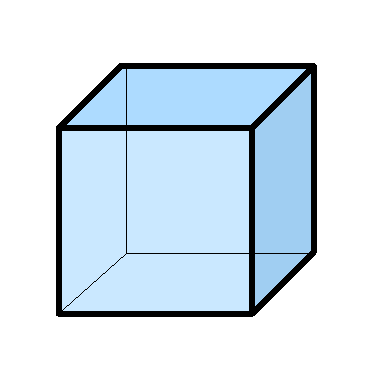
\includegraphics[height=3cm]{figs/homogeneous_bold-box.pdf}
   %\caption{A homogeneous number density profile $n(\vec{r})$.}
   %\label{fig:homogen_denisty}
%\end{figure}


%\begin{frame}{Gaussians in a primitive cell}
    %\begin{figure}
       %\centering
       %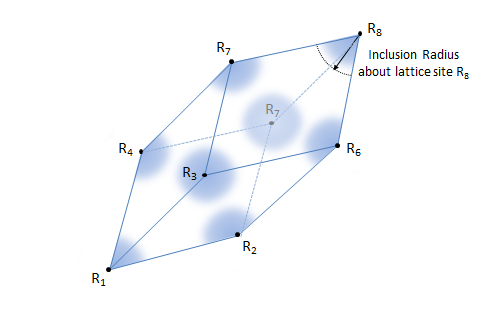
\includegraphics[height=5cm]{InclusionRadius.png}
       %%\caption{Gaussians are centered at each lattice point. After a radius 
       %%of a few Gaussian widths about each lattice point, the Gaussians go to 
       %%zero and can be neglected.}
       %%\label{fig:InclusionRadius}
    %\end{figure} 
%\end{frame}


%\begin{frame}{Maxwell's Double Tangent Construction}     
    %\begin{figure}
      %\centering
       %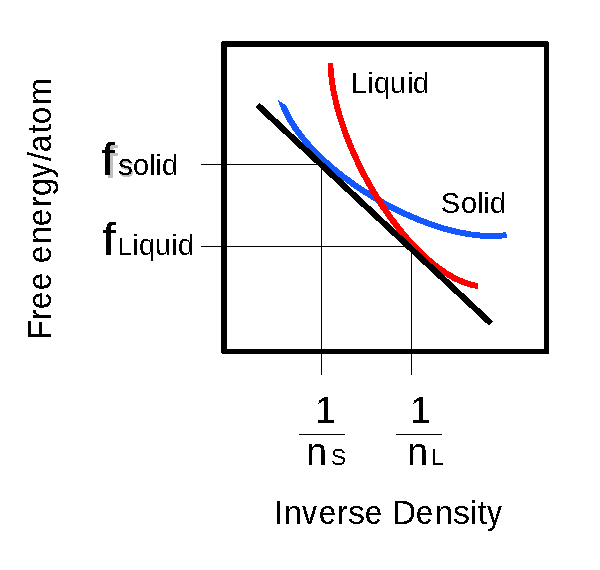
\includegraphics[height=6cm]{figs/MaxwellDTC-Fig1.pdf}
      %%\caption{Liquid and solid densities at the solid-liquid phase 
      %%transition are identified using Maxwell's Double Tangent Construction}
    %\end{figure}    
%\end{frame}



\subsection*{WCA Phase diagrams}

\begin{frame}{Temperature-Density Phase Diagram}
\begin{columns}
    \column{.5\textwidth}
	    \vspace{-2em}
        \begin{block}{}
            \begin{itemize}
              \item Data shown for dimensionless temperatures from $K_BT=~$0.5 to 3.0
              \item Freezing indicated by 
            
               presence of coexistence
            
               region, abrupt change 
            
               in density!
              \item Nearly matches results from Monte-Carlo simulations, 
              
              coexistence region at slightly higher densities
            \end{itemize}
            \end{block}
       \column{.65\textwidth}
    \begin{figure}
        \centering
        \includegraphics[width=.9\columnwidth]{figs/Phase_Diagram_of_T_vs_n}\\
    \end{figure}        
    \vspace{-1em}
    \footnotesize $~~~~~~~~~~~~$Monte-Carlo data from Chris May, 
    
     $~~~~~~~~~~~~$OSU undergraduate thesis
     \normalsize
     \end{columns}
\end{frame}

\begin{frame}{Pressure-Temperature Phase Diagram}
\begin{columns}
   \column{.5\textwidth}
	    \vspace{-2.2em}
        \begin{block}{}
            \begin{itemize}
            \item Data shown for dimensionless temperatures from $K_BT=~$0.5 to 3.0
            \item Freezing at phase boundary
            \item Does not closely match 
            
            results from Monte-Carlo simulations 
            \item Discrepancy gets worse as pressures and temperatures increase
            \end{itemize}
            \end{block}
       \column{.65\textwidth} 
         \begin{figure}       
           \centering
            \includegraphics[width=.9\columnwidth]{figs/Phase_Diagram_of_P_vs_T}\\
          \end{figure}  
        \vspace{-1em}
        \footnotesize $~~~~~~~~~~~~$Monte-Carlo data from Chris May, 
    
         $~~~~~~~~~~~~$OSU undergraduate thesis
        \normalsize
     \end{columns}
\end{frame}


\begin{frame}{What we have done}
       %\vspace{-2em}
        \begin{block}{Constructed a functional for a WCA fluid using cDFT}
            \begin{itemize}
              \item Gaussian weighted-density  
              \item Temperature dependent parameters designed to fit WCA fluid
           \end{itemize}
        \end{block}
        \begin{block}{Created an array of number density profiles to model crystal}
           \begin{itemize}
              %\item to model a crystal
              \item Consists of a sum of Guassian distributions %centered at lattice sites
              \item Vary by changing width and fraction of vacancies
           \end{itemize}
         \end{block}
         \begin{block}{Constructed T-n, and P-T phase diagrams}
           \begin{itemize}
              \item Showed freezing of WCA fluid over broad range of temperatures
              \item Farily good match with Monte-Carlo simulations
           \end{itemize}
         \end{block}
\end{frame}




%\begin{frame}{Conclusions and Further Research}
          %\begin{block}{Some things we could do}
            %\begin{itemize}
            %\item We have constructed a functional for a WCA fluid by creating 
            %temperature dependent parameters that fit the functional 
            %to the WCA fluid
            %\item 
            %\item
            %\end{itemize}
         %\end{block}
%\end{frame}


\end{document}

%\begin{frame}{What we have done}
%\vspace{-2em}
        %\begin{block}{}
            %\begin{itemize}
            %\item We have constructed a functional for a WCA fluid 
            
            %using cDFT by using a Gaussian weighted-density, 
            
            %and
            %creating temperature dependent 
            %parameters 
            
            %to fit the functional to a WCA fluid.
            %\item We have created an array of number density profiles 
            
            %to use in the functional to model a crystal, which 
            
            %consist of a sum of Guassian distributions centered at lattice sites,
            
            %which are varied in width and by vancancies.
            %\item We have constructed T-n, and P-T phase diagrams which 
            %show freezing of a WCA fluid over a broad range of temperatures
            %\end{itemize}
         %\end{block}
%\end{frame}


%Chris's old stuff...
%\section*{Next section}
%\begin{frame}{What is free energy?}
	%\begin{block}{Intuitive}
			%$F$ - the available work in the system
	%\end{block}
    %\begin{block}{Mathematics}
		%\vspace{1em}
		%\begin{columns}[t]
		%\column{.5\textwidth}		
		%{\centering Thermodynamics:
		%\begin{align*}
			%\diff F &= - S\,  \diff T + P\, \diff V
		%\end{align*}}
		%\column{.5\textwidth}
		%{\centering
		%Statistical Mechanics
		%\begin{align*}
		%F &= - k_B T \ln Z
		%\end{align*}}
		%\end{columns}
    %\end{block}		
		%Why Helmholtz and not Gibbs?
	%\begin{itemize}
		%\item Control temperature and volume 
		%\item Entropy a more preferable partial derivative
	%\end{itemize}
%\end{frame}

%\subsubsection*{Excess}
%\begin{frame}{Excess free energy}	
	%\begin{columns}[t]
	%\setlength\abovedisplayskip{-2pt} 
	%\column{.4\textwidth}	
	%\begin{align*}
		%Z_{exc} &= \int_s \frac{\diff\mathbf{r}^N}{V^N} ~e^{-\beta \Phi(\mathbf{r_1}, \mathbf{r_2}, \dots \mathbf{r_N})}
	%\end{align*}
	%\begin{itemize}
		%\item No algebraic expression for even simple $\Phi$
		%\item Need to use models, simulations to approximate behavior
		%\item Even with models...
	%\end{itemize}
	%\column{.6\textwidth}
	%\begin{figure}
		%\caption{Hard sphere and square well intermolecular pair potentials.}
	%\end{figure}
	%\end{columns}
%\end{frame}


%\subsection*{Methods}
%\begin{frame}{Methods}
	%\begin{itemize}
		%\item Thermodynamic Integration: integration over densities
		%\item Square Well Monte Carlo: integration over temperature
	%\end{itemize}
%\end{frame}

%\subsection*{Results}
%\begin{frame}{Results}
%\begin{columns}
	%\column{.7\textwidth}
        %FIXME the file figs/Fabs-vs-eta is missing
	%%% \frame{\includegraphics[width=\textwidth]{figs/Fabs-vs-eta}}
	%\column{.4\textwidth}
	%\begin{itemize}
		%\item Two doubling regimes simulated
		%\item Becomes more negative with increasing temperature, density 
	%\end{itemize}
%\end{columns}
%\end{frame}

%\section*{Final thoughts}
%\subsection*{Remarks}
%\begin{frame}{Remarks}
	%\begin{itemize}
		%\item Liquids - however simple - are very complicated
		%\item Simplest models have no analytic solutions
		%\item Separation enables some behavioral investigation
	%\end{itemize}
%\end{frame}
%\subsection*{References}
%\begin{frame}{References}
	%\tiny
	%\begin{itemize}
		%\item Retrieved from \url{https://nicokrisch.files.wordpress.com/2014/05/}
		%\item Retrieved from \url{https://en.wikipedia.org/wiki/Chemical_polarity}
		%\item I. M. J.-P. Hansen, Theory of Simple Liquids, $3^{\text{rd}}$ ed. (Academic Press, 2006).
		%\item M. A. Perlin, ``Optimizing monte carlo simulation of the square-well fluid,'' (2015), Oregon State University.
		%\item A. Valeske, ``Determining free energies of hard sphere fluids via monte carlo simulation'' (2015), Oregon State University.
	%\end{itemize}
%\end{frame}

